%%%%%%%%%%%%%%%%%%%%%%%%%%%%%%%%%%%%%%%%%
%
% (c) 2018 by Jennifer Laaser
%
% This work is licensed under the Creative Commons Attribution-NonCommercial-ShareAlike 4.0 International License. To view a copy of this license, visit http://creativecommons.org/licenses/by-nc-sa/4.0/ or send a letter to Creative Commons, PO Box 1866, Mountain View, CA 94042, USA.
%
% The current source for these materials is accessible on Github: https://github.com/jlaaser/pogil-polymers
%
%%%%%%%%%%%%%%%%%%%%%%%%%%%%%%%%%%%%%%%%%

\renewcommand{\figpath}{content/polymchem/stepgrowth/dispersity/figs}

\begin{activity}[Molecular Weight Distributions in Step-Growth Polymerizations]

\begin{instructornotes}

	This activity introduces students to key concepts related to the molecular weight distributions obtained in step-growth polymerizations.
	
	After completing this activity, students will be able to:
			\begin{enumerate}
				\item Calculate the fraction of polymer chains with length $i$ in a step-growth polymerization,
				\item Describe, qualitatively, the chain length distribution and how it changes with extent of reaction,
				\item Calculate the expected dispersity for step-growth polymerizations, and
				\item Explain why the limiting dispersity for a step-growth polymerization is 2.
			\end{enumerate}
			
	\subsection*{Activity summary:}
	\begin{itemize}
		\item \textbf{Activity type:} Learning Cycle
		\item \textbf{Content goals:} Molecular weight distributions and dispersity in step-growth polymerizations
		\item \textbf{Process goals:} %https://pogil.org/uploads/attachments/cj54b5yts006cklx4hh758htf-process-skills-official-pogil-list-2015-original.pdf
			written communication, critical thinking, information processing
		\item \textbf{Duration:} 25-30 minutes, including time for discussion
		\item \textbf{Instructor preparation required:} none beyond knowledge of relevant content
		\item \textbf{Related textbook chapters:}
			\begin{itemize}
				\item \emph{Polymer Chemistry} (Hiemenz \& Lodge): section 2.4
			\end{itemize}
	\end{itemize}

\end{instructornotes}

	%\textbf{Focus question:} Put a central question for the students to consider through this exercise here.

\begin{model}[Probabilities of Forming Different Chain Lengths]

Suppose we perform a step-growth polymerization of AB-type monomers and stop the polymerization at extent of reaction $p$ (i.e. we stop the polymerization when the fraction of A groups that have reacted is equal to $p$).

Suppose we then select a single molecule from this reaction mixture.  This molecule will have an unreacted A group on one end, and an unreacted B group on the other.

Consider the following argument:
\begin{enumerate}
\item The unreacted `B' group was originally part of an `AB' monomer. Of these AB monomers ($i=1$),
\begin{itemize}
	\item The fraction in which the A group monomer did \textit{not} react, and the molecule remained an AB monomer, is $1-p$.

	\item The fraction in which the A group \textit{did} react, and the selected molecule is at least an AbaB dimer, is $p$.
\end{itemize}

\item Of the molecules that reacted to form AbaB dimers ($i=2$),
\begin{itemize}
	\item The fraction \emph{of dimers} in which the A group did not react, and the molecule remained an AbaB dimer, is $1-p$. The total fraction \emph{of molecules} that are AbaB dimers is thus 
	\begin{gather*}(\text{\small fraction of molecules that form dimers})\cdot(\text{\small fraction of dimers that don't react further})\\ =p(1-p)\end{gather*}

	\item The fraction \emph{of dimers} in which the A group did react, and the selected molecule is at least an AbabaB trimer, is $p$. The total fraction \emph{of molecules} that form at least an AbabaB trimer is thus 
	\begin{gather*}(\text{\small fraction of molecules that form dimers})\cdot(\text{\small fraction of dimers that react further}) \\= p\cdot p=p^2 \end{gather*}
\end{itemize}

\item Of the molecules that reacted to form AbabaB trimers ($i=3$),
\begin{itemize}
	\item The fraction \emph{of trimers} in which the A group did not react, and the molecule remained an AbabaB trimer, is $1-p$. The total fraction \emph{of molecules} that are AbabaB trimers is thus 
	\begin{gather*}(\text{\small fraction of molecules that form trimers})\cdot(\text{\small fraction of trimers that don't react further})\\ =p^2(1-p)\end{gather*}

	\item The fraction \emph{of trimers} in which the A group did react, and the selected molecule is at least an AbababaB tetramer, is $p$. The total fraction \emph{of molecules} that form at least an AbababaB tetramer ($i=4$) is thus 
	\begin{gather*}(\text{\small fraction of molecules that form trimers})\cdot(\small \text{fraction of trimers that react further}) \\= p^2\cdot p=p^3 \end{gather*}
\end{itemize}

%We can represent this tree of probabilities graphically as follows:
\end{enumerate}

%\vspace{0.1in}
%\centerline{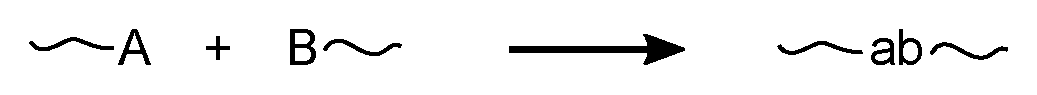
\includegraphics[width=0.6\textwidth]{\figpath/ABrxn.pdf}}

\end{model}

\vspace{0.05in}
\begin{ctqs}

	\question Following this reasoning, 
	
		\begin{enumerate}
			\item How would you calculate the fraction of \emph{molecules} that \emph{remain} as AbababaB tetramers ($i=4$)?  Write your answer in both words and symbols.
	
				\begin{solution}[1.25in]
					The fraction of molecules that remain as tetramers is
	\begin{gather*}(\text{\small fraction of molecules that form tetramers})\cdot(\text{\small fraction of tetramers that don't react further})\\ =p^3(1-p)\end{gather*}
				\end{solution}
			
			\item How would you calculate the fraction of molecules that react further to form at least an AbabababaB pentamer ($i=5$)? Write your answer in both words and symbols.
			
				\begin{solution}[1.25in]
					The fraction of molecules that reacted to form at least a pentamer is 
	\begin{gather*}(\text{\small fraction of molecules that form tetramer})\cdot(\small \text{fraction of tetramers that react further}) \\= p^3\cdot p=p^4 \end{gather*}
				\end{solution}
		
		\end{enumerate}
	
	\question Using the information in the model, and your answers to the previous question, fill in the following table:
	
		\begin{center}
			\renewcommand{\arraystretch}{3.5}
			\begin{tabular}{|c|c|}
				\hline
				\textbf{~~i~~} & {\renewcommand{\arraystretch}{1}\begin{tabular}{c}\textbf{Fraction of molecules that contain}\\\textbf{exactly $i$ monomers}\end{tabular} }\\\hline
				1 & \answer{$1-p$}\\\hline
				2 & \answer{$p(1-p)$}\\\hline
				3 & \answer{$p^2(1-p)$}\\\hline
				4 & \answer{$p^3(1-p)$}\\\hline
				5 & \answer{$p^4(1-p)$}\\\hline
			\end{tabular}
		\end{center}
	
	\question What pattern do you notice in these values?  Briefly describe your observations in 1-2 complete sentences.
	
		\begin{solution}[1in]
		
			The values acquire an additional factor of $p$ for each additional monomer in the chain.
		
		\end{solution}
	
	\question Complete the following statement:
	
		``The fraction of molecules, $x_i$, that are composed of exactly $i$ monomers is \line(1,0){50}.''
	
		\begin{solution}[0.5in]
		
			$x_i = p^{i-1}(1-p)$
			
		\end{solution}
	
	\question Using this expression, calculate the fraction of molecules that have exactly length $i$ for both $p=0.5$ and $p=0.9$ at the following values of $i$:
	
		\begin{center}
			\renewcommand{\arraystretch}{4}
			\begin{tabular}{|c|c|c|}
				\hline
				\textbf{~~$i$~~} & ~~~$x_i$ when $p=0.5$~~~ & ~~~$x_i$ when $p=0.9$~~~ \\\hline
				1 & \answer{0.5} & \answer{0.1} \\\hline
				2 & \answer{0.25} & \answer{0.09} \\\hline
				3 & \answer{0.125} & \answer{0.08} \\\hline
				5 & \answer{0.0313} & \answer{0.065} \\\hline
				10 & \answer{9.7x10$^{-4}$} & \answer{0.0387} \\\hline
				15 & \answer{3.1x10$^{-5}$} & \answer{0.0229} \\\hline
				20 & \answer{9.5x10$^{-7}$} & \answer{0.0135} \\\hline
			\end{tabular}
		\end{center}
		
		\clearpage
	\question Plot your results on the following axes.  Make sure to use a different symbol for points corresponding to $p=0.5$ than for the points corresponding to $p=0.9$.
	
		\begin{solution}[2.75in]
			\studentdisplay{
				\centerline{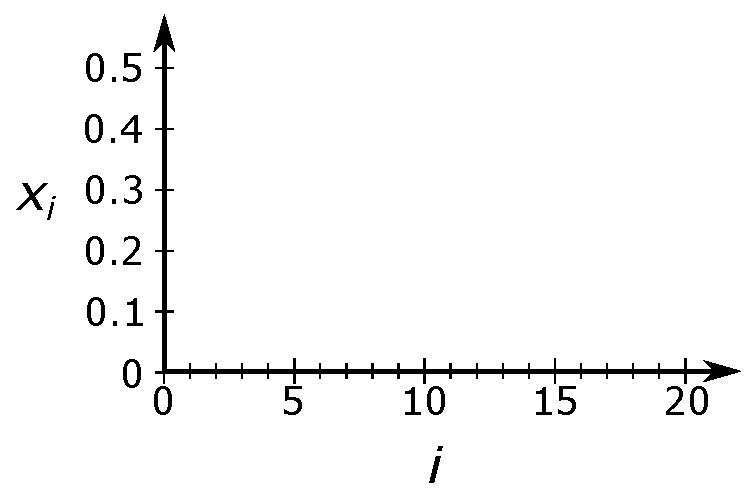
\includegraphics[width=0.7\textwidth]{\figpath/model1-xi-axes.pdf}}
			}
			\instructordisplay{
				\centerline{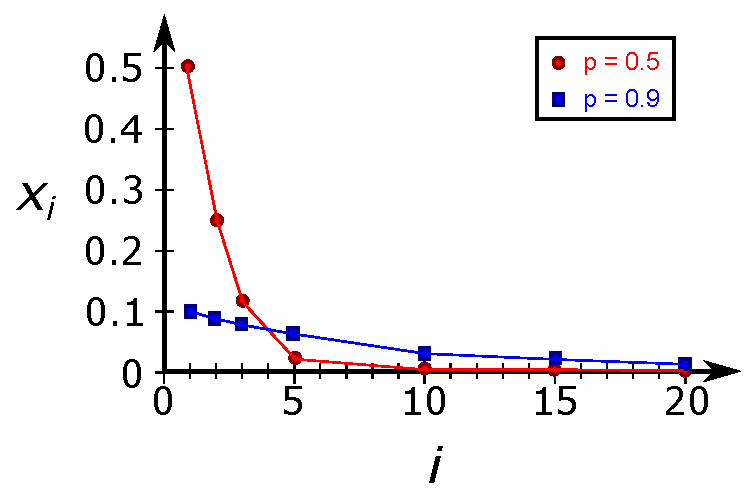
\includegraphics[width=0.7\textwidth]{\figpath/model1-xi-plotted.pdf}}
			}
		\end{solution}
	
	\question How are the plots for $p=0.5$ and $p=0.9$ similar, and how are they different?  Briefly describe your observations in 2-3 complete sentences.
	
		\begin{solution}[1.5in]
		
			Both of these plots decrease exponentially toward zero with increasing values of $i$.  However, the plot for $p=0.5$ decreases much faster, and a higher fraction of the molecules have very short chain lengths, than in the case where $p=0.9$.
		\end{solution}
	
	\question What is the \emph{most probable} chain length for each value of $p$?
	
		\begin{solution}[0.5in]
		
			The most probable chain length is just the one with the highest value of $x_i$.  Thus, the most probably chain length is $i=1$ for both values of $p$.
		
		\end{solution}
	
	\question Can the fraction of chains with length $i+1$ ever be \emph{greater} than the fraction of chains with length $i$?  Justify your answer in 1-2 complete sentences.
	
		\begin{solution}[1.5in]
		
			No, the fraction of chains with length $i+1$ can never be greater than the mole fraction of chains with length $i$.  This is because for each additional monomer, we pick up another factor of $p$; since $p$ is always less than one, $x_{i+1}$ will always be less than $x_i$.
			
			In mathematical terms, $x_i$ decreases monotonically with increasing chain length $i$.
		
		\end{solution}
	
\end{ctqs}


\begin{model}[$M_n$ and $M_w$ for Step-Growth Polymerizations]

	To calculate $M_n$ and $M_w$, we need to know $n_i$, or the total number of chains with $i$ monomers.
	
	If we started with $v_A^0$ monomers, then when the extent of reaction is equal to $p$, there will be $(1-p)v_A^0$ unreacted A groups left.  Recalling that the number of unreacted A groups is equal to the number of molecules in the reaction mixture, this lets us write
	\begin{align*}
		n_i &= \text{(fraction of molecules that have length }i\text{) x (number of molecules in reaction mixture)}\\
			%&= (x_i)((1-p)v_A^0)\\
			&= \left(p^{i-1}(1-p)\right)\left((1-p)v_A^0\right)\\
			&= p^{i-1}(1-p)^2v_A^0
	\end{align*}
	
	If we plug this expression into our equation for $M_n$, we get
	\begin{equation*}
		M_n = \frac{\sum_i n_i M_i}{\sum_i n_i} %= \frac{\sum_i p^{i-1}(1-p)^2 v_A^0 i M_0}{\sum_i p^{i-1}(1-p)^2 v_A^0} 
		= M_0\frac{\sum_i p^{i-1}(1-p)^2 i }{\sum_i p^{i-1}(1-p)^2}
	\end{equation*}
	where $M_0$ is the molecular weight of the monomer ($M_i = M_0 i$).
	
	\vspace{0.25in}
	
	Evaluating these sums is a bit tedious, but if we do so, we obtain
	\begin{align*}
		M_n = \frac{M_0}{1-p} && \text{or} && N_n = \frac{M_n}{M_0} = \frac{1}{1-p}
	\end{align*}
	which is exactly what we expected (whew - our math worked!).
	
	\vspace{0.25in}
	Similarly, if we plug this expression into our equation for $M_w$ and work through the sums, we get
	\begin{align*}
		M_w = \frac{\sum_i n_i M_i^2}{\sum_i n_i M_i} = M_0\frac{1+p}{1-p} && \text{or} && N_w = \frac{M_w}{M_0} = \frac{1+p}{1-p}
	\end{align*}

\end{model}

\begin{ctqs}
		\question Calculate the dispersity for a step-growth reaction with extent of reaction $p$.
		
			\begin{solution}[1.95in]
			
				\begin{equation*}
					\text{\DJ} = \frac{M_w}{M_n} = \frac{M_0\frac{1+p}{1-p}}{M_0\frac{1}{1-p}} = 1+p
				\end{equation*}
			\end{solution}
			
			
		\question What is the value of the dispersity when $p=0$?  Briefly comment on whether or not this answer makes sense.
		
			\begin{solution}[1.5in]
			
				When $p=0$, $\text{\DJ}=1+0 = 1$.  This does make sense: when the extent of reaction is zero, no reactions have taken place, and the reaction mixture contains only monomers.  Since all of the molecules in the mixture are thus identcail (and exactly the same size), the dispersity is 1 - the mixture is monodisperse.
			
			\end{solution}
			
			
		\question What is the value of the dispersity when $p=1$?
		
			\begin{solution}[1in]
			
				When $p=1$, $\text{DJ}=1+1=2$.  This is an important limit: the limiting dispersity for a step-growth polymerization is 2.
			
			\end{solution}
			
			
			
		\question Can the dispersity of a polymer produced by step-growth polymerization ever be greater than 2?  Briefly defend your answer in 1-2 complete sentences.
		
			\begin{solution}[1.5in]
			
				Following the argument presented in this exercise, no, the dispersity of a polymer produced by step-growth polymerization can never be greater than 2, because $p$ can never be greater than 1. 
				
				Note for instructors: practically speaking, there are certain conditions that can generate dispersities greater than 2 (for example, when the reaction mixture contains multifunctional monomers that induce chain branching, or when the monomers are added in several batches - see DOI:10.1016/0032-3861(92)90340-3), but for the purposes of this activity, students should learn that the ideal limiting dispersity for step-growth polymerizations is two.
			
			\end{solution}
			
			
\end{ctqs}

\begin{exercises}

		\exercise Suppose you synthesized a polymer by step-growth polymerization and found that it had a dispersity of 1.86.
		
			\begin{enumerate}
				\item What must the extent of reaction have been in this polymerization?
		
					\begin{solution}
					\instructordisplay{
						\begin{equation*}
							p = \text{\DJ}-1 = 1.86-1 = 0.86
						\end{equation*}
					}
					\end{solution}
					
				\item What would you expect the number-average degree of polymerization of this polymer to be?
		
					\begin{solution}
					\instructordisplay{
						\begin{equation*}
							N_n = \frac{1}{1-p} = \frac{1}{1-0.86} = 7.1
						\end{equation*}
					}
					\end{solution}
			\end{enumerate}
			
\end{exercises}
	
\end{activity}